\documentclass[11pt,a4paper]{article}

\usepackage{amsfonts}
\usepackage{amssymb}

\usepackage{amsthm}
\usepackage{epsfig}
\usepackage{graphicx}
\usepackage{natbib}		% citet, citep
\usepackage{textcomp}
\usepackage{booktabs}
\usepackage{multirow}
\usepackage{fullpage}
\usepackage{authblk}
\usepackage{url}
\usepackage{color}
\usepackage{tikz}
\usepackage{float}
% \usepackage{xeCJK}
% \setCJKmainfont{TW-Kai} 

% use for game tree
\usepackage{amsmath}
\def\vpay#1#2{\begin{matrix}#1\\#2\end{matrix}}
\usepackage{istgame}

\renewcommand{\baselinestretch}{1.4}

\parskip=5pt
\parindent=20pt
\footnotesep=5mm

\newtheorem{lem}{Lemma}
\newtheorem{prop}{Proposition}
\newtheorem{defn}{Definition}
\newtheorem{cor}{Corollary}
\newtheorem{ass}{Assumption}
\newtheorem{obs}{Observation}
\newenvironment{pf}{\begin{proof}\vspace{-10pt}}{\end{proof}}
% \newtheorem{ques}{Question}
% \newtheorem{rmk}{Remark}
% \newtheorem{note}{Note}
% \newtheorem{eg}{Example}

\newenvironment{enumerateTight}{\begin{enumerate}\vspace{-8pt}}{\end{enumerate}\vspace{-8pt}}
\newenvironment{itemizeTight}{\begin{itemize}\vspace{-8pt}}{\end{itemize}\vspace{-8pt}}
\leftmargini=25pt   % default: 25pt
\leftmarginii=12pt  % default: 22pt

\DeclareMathOperator*{\argmax}{argmax}
\DeclareMathOperator*{\argmin}{argmin}
\setcounter{MaxMatrixCols}{20}

\title{Computer Network and Application (110-1) \\ Homework 3}

\author{Minchun Chen (B08705051)}
\date{}

\begin{document}

\maketitle

\section{R4}
TCP is reliable, but slower compared to UDP. So when the application needs fast transfer speed, and some packet loss 
is tolerable, the application developer might choose UDP over TCP.\\
For example, live streaming needs packets to arrive as fast as possible, and some loss is fine as long as user can
watch the stream without lagging. Thus, the application developer might choose UDP over TCP in this case.

\section{R6}
I think the answer is positive, but it'll be harder to achieve reliability on UDP than on TCP, since we have to 
implement reliable transfer on the application layer. The application needs to assure that every data segment is 
received and ordered, and ask for server to re-transmit loss packets.

\section{R10}
Timers are introduced to detect packet loss. If a ACK message isn't received with the duration of the timer, the packet 
(or the ACK) is assumed to be lost. Then, the server would re-transmit the packet.

\section{P8}
\begin{figure}[H]
    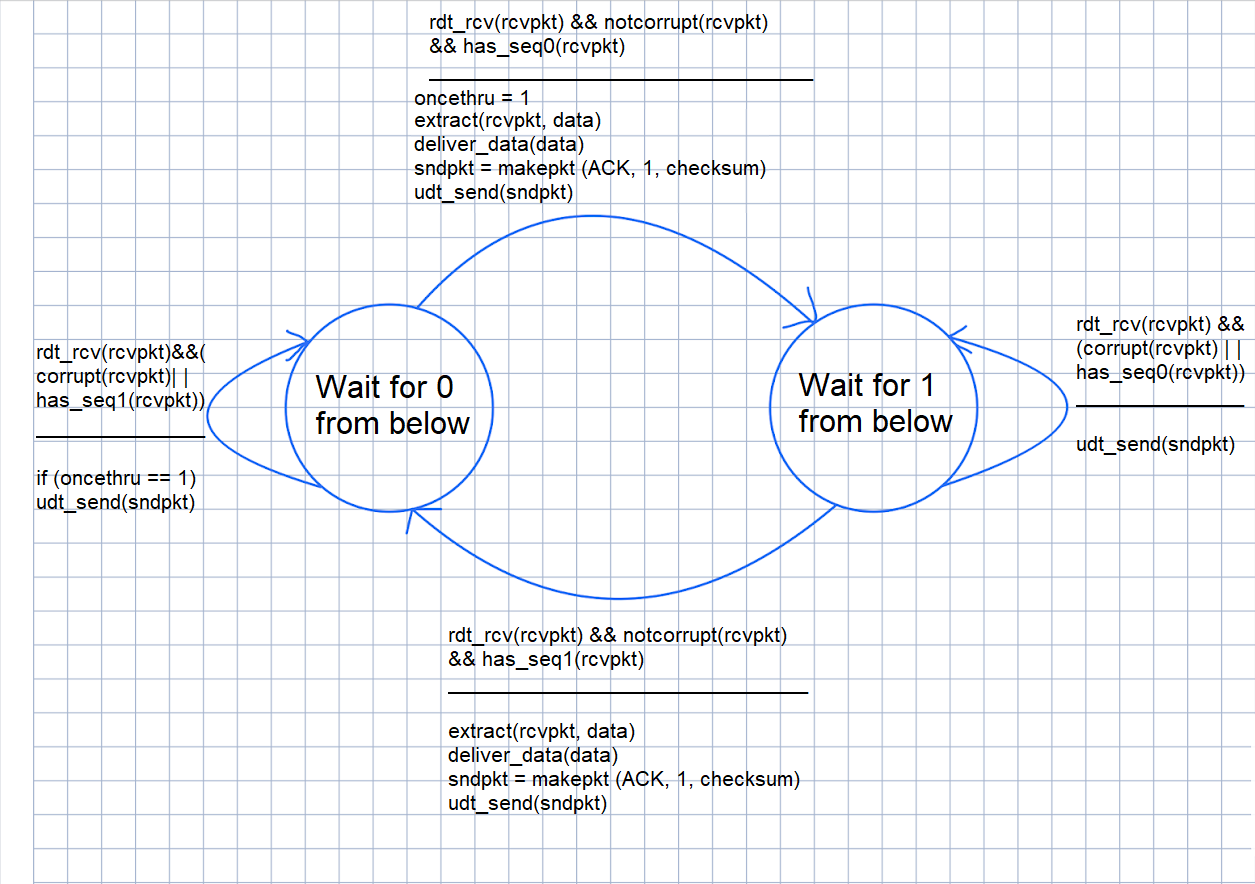
\includegraphics[width=\linewidth]{./rdt_receiver.png}
    \caption{rdt3.0 receiver FSM}
    \label{rdt_receiver}
\end{figure}

\section{P10}
\begin{figure}[H]
    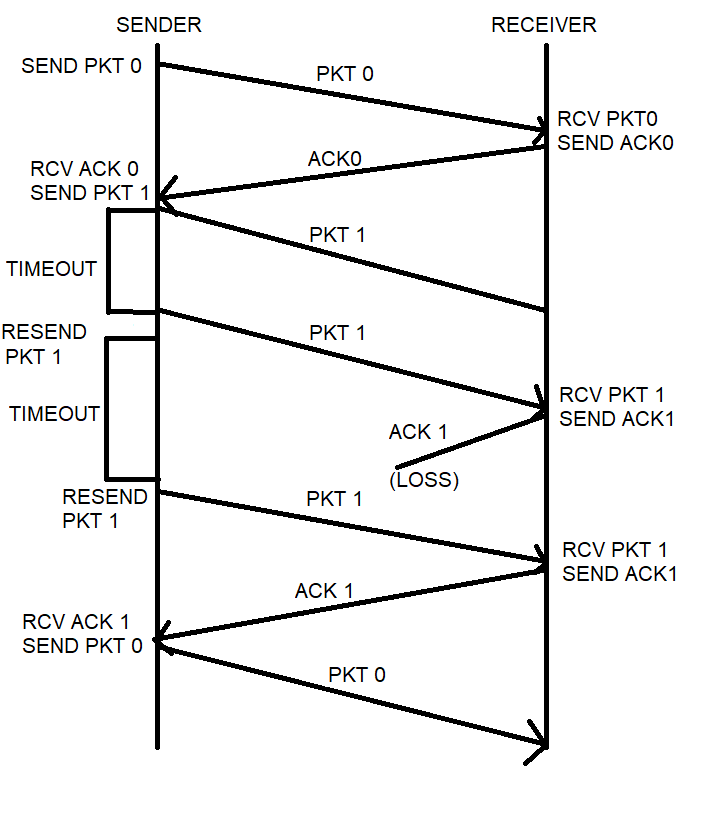
\includegraphics[width=\linewidth]{./rdt2.1_sender_timeout.png}
    \caption{rdt2.1 modified}
    \label{rdt_sender}
\end{figure}

\section{P13}
With TCP, it'll adjust sutomatically with its congestion control algorithm. But with UDP, you have to detect congestion 
and adjust your transmission rate in the application layer. \\
Another option is that the router can send message telling edge devices that a congestion has occured, so that they can
adjust transmission rate and mitigate the congestion situation.

\section{P15}
Suppose the round trip time between A and B is 20ms. \\
Transmission rate of the link is 500 Mb = $5 \times 10^8$ bps.

$$ D_{trans} = \frac{L}{R} = \frac{1500 \times 8}{5 \times 10^8} = 2.4 \times 10^{-5} s$$ \\
Suppose that window size is $N$\\
Channel Utilisation = 
\begin{align*}
    N \times \frac{L/R}{ L/R + RTT } &= \frac{98}{100} \\
    N \times \frac{0.024}{20 + 0.024} &= \frac{98}{100} \\
    2.4 \times N &= 98 \times 20.024 \\
    N &= 817.64
\end{align*}

Therefore, to utilize $98\%$ of the channel, the window size should be 818 packets approximately.

\end{document}